%---------------------导言区---------------------------%
\documentclass[10pt,a4paper,twoside,UTF8]{ctexart}
\usepackage{geometry}%用于设置上下左右页边距
	\geometry{left=2cm,right=2cm,top=2.5cm,bottom=3cm}
\usepackage{xeCJK,amsmath,paralist,enumerate,booktabs,multirow,graphicx,subfig,setspace,listings}
	\setlength{\parindent}{2em}%正文首行缩进两个汉字
	\lstset{language=tex}
\usepackage{titlesec}
	\newfontfamily\sectionef{Times New Roman}
	\setCJKfamilyfont{FZHeiTi}{黑体}
	\newcommand{\sectioncf}{\CJKfamily{FZHeiTi}}
	\titleformat*{\section}{\large\bfseries\sectioncf\sectionef}
	\titleformat*{\subsection}{\normalsize\bfseries\sectioncf\sectionef}
\usepackage{fancyhdr}
\usepackage{float}
\usepackage{layout}
\setlength{\skip\footins}{0.5cm}%脚注与正文的距离
\renewcommand{\footnotesize}{}%设置脚注字体大小
\setlength\columnsep{0.8cm}%设置双栏的间距
\usepackage{ifthen}%这个宏包提供逻辑判断命令
\newboolean{first}%引入布尔变量
\setboolean{first}{true}%将布尔变量设置为true
\pagestyle{fancy}
	\fancypagestyle{maincontent}{
		\fancyhf{}  %清空页眉页脚设置
		\fancyhead[EL, OR]{\thepage}
		\fancyhead[EC]{实验C9 混沌电路实验}
		\fancyhead[OC]{基\quad 础\quad 物\quad 理\quad 实\quad 验}
		\renewcommand\headrulewidth{0pt}
	}

	\usepackage{chngcntr}
	\counterwithin{figure}{section}
	\usepackage{datetime}
	\fancypagestyle{firstpage}{
		\setboolean{first}{false}%firstpage出现,则将first重置为false
		\fancyhf{}  %清空页眉页脚设置
		\fancyhead[L]{\the\year 年\the\month 月}
		\fancyhead[R]{\shortmonthname[\the\month], \the\year}
		\fancyhead[C]{
		\large{基\quad 础\quad 物\quad 理\quad 实\quad 验}\\
		\normalsize{GENERAL PHYSICS LABORATORY}
		}
	}

	%%% Step3 页眉线的设置:用布尔变量区分首页和正文
	\newcommand{\makefirstpageheadrule}{%定义首页页眉线-双线绘制命令
	\makebox[0pt][s]{\rule[0.6\baselineskip]{\headwidth}{0.3pt}}
	\makebox[0pt][s]{\protect\hspace{-0.34em}\rule[0.75\baselineskip]{\headwidth}{0.3pt}}
	\protect\vspace{-20pt}
	}

	\newcommand{\makeheadrule}{%定义正文页页眉线绘制命令,单线
	\makebox[0pt][l]{\rule[1\baselineskip]{\headwidth}{0.3pt}}
	\protect\vspace{-20pt}%页眉和正文的距离
	}

	%根据布尔变量first为true或false分别执行不同的页眉线绘制命令
	\renewcommand{\headrule}{%重定义headrule命令
	\ifthenelse{\boolean{first}}{\makeheadrule}
	{\makefirstpageheadrule}
	}
%%end--------------设置首页和正文不同的页眉页脚-----------%%



%%begin-----------------参考文献-----------------------%%
% \usepackage{cite}
% \newcommand{\upcite}[1]{\textsuperscript{\textsuperscript{\cite{#1}}}} %参考文献上标
%\usepackage[backref]{hyperref}
\usepackage{url}
\usepackage[colorlinks,linkcolor=blue,urlcolor=blue]{hyperref}%超链接
\usepackage[hyperref=true,backend=biber,bibstyle=gb7714-2015,citestyle=numeric-comp,sorting=none,backref=true]{biblatex}
	%hyperref=true和backref=true表示为各个参考文献的引用处、及定理、定义、例子等的引用处都添加上超链接;
	%backend=biber:后端处理的程序为biber.exe
	%bibstyle:参考文献风格;每个期刊、组织要求不同
		%gb7714-2015是目前国内期刊通用的风格,称为gb标准风格
	%citestyle:引用风格;每个期刊、组织要求不同
	%sorting=none:按照参考文献在论文中出现的先后顺序排序。
	%**编译:biblatex与biber命令配合使用。xelatex-biber-xelatex-xelatex
\addbibresource{ref.bib}
	%这里写上.bib文件的相对地址
	%每次实验引用的页数不同,需要手动改变


	\usepackage{listings}
	\usepackage{color}
	
	\definecolor{dkgreen}{rgb}{0,0.6,0}
	\definecolor{gray}{rgb}{0.5,0.5,0.5}
	\definecolor{mauve}{rgb}{0.58,0,0.82}
	
	\lstset{ %
	  language=Python,                % the language of the code
	  basicstyle=\footnotesize,           % the size of the fonts that are used for the code
	  numbers=left,                   % where to put the line-numbers
	  numberstyle=\tiny\color{gray},  % the style that is used for the line-numbers
	  stepnumber=1,                   % the step between two line-numbers. If it's 1, each line 
									  % will be numbered
	  numbersep=5pt,                  % how far the line-numbers are from the code
	  backgroundcolor=\color{white},      % choose the background color. You must add \usepackage{color}
	  showspaces=false,               % show spaces adding particular underscores
	  showstringspaces=false,         % underline spaces within strings
	  showtabs=false,                 % show tabs within strings adding particular underscores
	  frame=single,                   % adds a frame around the code
	  rulecolor=\color{black},        % if not set, the frame-color may be changed on line-breaks within not-black text (e.g. commens (green here))
	  tabsize=2,                      % sets default tabsize to 2 spaces
	  captionpos=b,                   % sets the caption-position to bottom
	  breaklines=true,                % sets automatic line breaking
	  breakatwhitespace=false,        % sets if automatic breaks should only happen at whitespace
	  title=\lstname,                   % show the filename of files included with \lstinputlisting;
									  % also try caption instead of title
	  keywordstyle=\color{blue},          % keyword style
	  commentstyle=\color{dkgreen},       % comment style
	  stringstyle=\color{mauve},         % string literal style
	  escapeinside={\%*}{*)},            % if you want to add LaTeX within your code
	  morekeywords={*,...}               % if you want to add more keywords to the set
	}
	
%%end-------------------参考文献-----------------------%%
%%%%%%%%%%%%%%%%%%%%%%%%%%%%%%%%%%%%%%%%%%%%%%%%%%%%%%%%%%
%%%%%%%%%%%%%%%%%%%%%%%%%正文开始%%%%%%%%%%%%%%%%%%%%%%%%%%
%%%%%%%%%%%%%%%%%%%%%%%%%%%%%%%%%%%%%%%%%%%%%%%%%%%%%%%%%%

\begin{document}


%%begin-------------------中文摘要-----------------------%%
\title{\LARGE\textbf{实验C9 混沌电路实验}\footnotemark[1]}
\author{\large\textit{XXX\footnotemark[2]}
\\ \normalsize{(1. \textit{中山大学 物理学院,广东 广州 }510275)}}
\date{}%不显示日期


	%twocolumn: 双栏article下的单栏摘要
	\maketitle  %标题和作者
  	\renewcommand{\abstractname} {} %不显示摘要名字
	\begin{abstract}
	\vspace{-3em}
	% vspace:调整垂直空白,可以自己调整;缩小abstract和center(以及maketitle)的间距
	%\noindent %备用:摘要无缩进
	{\bf 摘{} 要:}
	{\small 
	混沌学属于非线性动力学,混沌理论认为混沌是在确定的非线性动力学
	系统中,不需要附加任何随机因素,在一定条件下就会呈现出类似随机但又遵循一定规
	律的复杂动力学振荡行为。
	利用电子电路的方法可以实现混沌振荡现象,本系列实验利用Python数值模拟,
	Multisim和LTspice软件仿真和NI Virtualbench交互式测量实际电
    路相结合的方法,观察若干种混沌现象,从理论和实践上还原了蔡氏和洛伦兹混沌电路。
	首先,本实验探究了不含电容蔡氏电路的不同混沌状态,从Python的数值模拟上看,第一种蔡氏电路可以得到直线、极限环、双吸引子、第一次和第二次
	单吸引子五种相图。通过Multisim仿真和全真电路均可以得到这五种相图。使用配对T检验对仿真和全真电路不同相图时同一电阻不同阻值进行分析,
	可以得到t值为-1.12901974098575,对应P值为0.322013731315691>0.05,无统计学差异,故得出结论仿真可以较好的模拟真实的第一种蔡氏混沌电路。
	其次,我们对含电容的蔡氏混沌电路进行Multisim仿真,分别出现直线、极限环、双吸引子和第一次单吸引子相图。
	通过搭建真实电路,使用NI Virtualbench ,同样可以出现这四种相图。
	经配对T检验得t值为-0.587714318298662,对应P值为0.598032391735953>0.05,无统计学差异,故得出结论仿真可以较好的模拟真实的第二种蔡氏混沌电路。
	最后,我们使用Python对经典洛伦兹混沌方程进行模拟,得到双吸引子的三维图、时域图和各平面投影图。使用LTspice仿真,当R2取不同阻值时,
	洛伦兹混沌电路的相图分别为直线、双吸引子和第一次单吸引子。若调节更多原件的参数,可能可以得到更多种类的相图。
}
	\par%空的新行的高度。
	\textbf{关键词}:混沌、蔡氏混沌电路、洛伦兹混沌电路、Multisim、LTspice、NI VirtualBench
	\vspace{2em}
	\end{abstract}

%%end--------------------英文摘要------------------------%%
\renewcommand{\thefootnote}{\fnsymbol{footnote}}
\footnotetext[1]{由中山大学物理学院陆佑堂提供器材和指导。}
\footnotetext[2]{作者简介:XXX,xxxxxxxx;E-mail: \url{xxxx@mail2.sysu.edu.cn}}

%%end-------------------中文摘要-----------------------%%


\thispagestyle{firstpage}%首页页面风格:firstpage
\pagestyle{maincontent}%第二页之后的页面风格:maincontent

%%begin------------------英文摘要------------------------%%

	\renewcommand{\abstractname} {} %不显示摘要名字
	\begin{center}%
		\begin{spacing}{2.0}
			{\LARGE\bfseries Experiment C9: Chaotic circuit experiment$^{*}$  }%
		\end{spacing}
	    \vskip 0.5em%
	    {\large
	    \lineskip .75em%
	    \begin{tabular}[t]{c}%
	    \large XXX$^{1}$
	    \end{tabular} 
	    }%
	    \vskip 0.4em%
	    {\normalsize 1. School of Physics, Sun Yat-sen University, Guangzhou  { \rm 510275}, China}
	\end{center}
	\begin{abstract}
		\vspace{-2em}  %缩小abstract和center(以及maketitle)的间距
	    	{\bf Abstract:}
	    {\small 
		Chaos belongs to nonlinear dynamics. chaos theory believes that chaos is in the determination of nonlinear dynamics.  
		In this system, there is no need to add any random factors, while under certain conditions will appear to be random.  
		The chaotic oscillation phenomenon can be constructed using electronic circuit method. This series of experiments used Python numerical simulation,  
		Multisim, LTspice software simulation and NI Virtualbench interactive measurement of real electricity.  
		Chua's and Lorentz's chaotic circuits were restored theoretically and practically by observing some chaotic phenomena.  
		First, this experiment explored the different chaotic states of the chua's circuit without capacitors. From the Python numerical simulation, the first Chua circuit can obtain straight lines, limit cycles, double attractors, first and second single attractors.
		These five phase diagrams can be obtained by Multisim simulation and full - truth circuit as well.  The pair-t test was used to analyze different resistance values of the same resistance in different phase diagrams of simulation and full true circuits.  
		It can be concluded that the T value is -1.12901974098575, and the corresponding P value is 0.322013731315691>0.05, which is of no statistical difference. Therefore, it can be concluded that the simulation can finely simulate the real first Chua's chaotic circuit.  
		Secondly, we did Multisim simulation for Chua's chaotic circuit with capacitor, and the phase diagrams of straight line, limit cycle, double attractor and first single attractor appeared respectively.  
		Using NI Virtualbench, these four diagrams can also appear by building real circuits.  
		The t-value obtained by paired T-test is -0.587714318298662, and the corresponding P-value is 0.598032391735953>0.05, showing no statistical difference. 
		Therefore, it is concluded that the simulation can finely simulate the real second Chua's chaotic circuit.  
		Finally, we used Python to simulate the classical Lorentz chaos equation. We got the 3d image, time domain image and plane projection image of the double attractor.  
		When R2 takes different resistance values,  
		The LTspice simulation phase diagrams of Lorentz chaotic circuit were linear, double attractor and first single attractor. 
		More types of phase diagrams may be obtained by adjusting the parameters of more elements.  }	    \par%空的新行的高度。
		\textbf{Key words}:Chaos, Chua's chaotic circuit, Lorentz chaotic circuit, Multisim, LTspice, NI VirtualBench
	\end{abstract}
	~\\



%%begin----------------层级结构------------------------%%

%重点1:知道每一个层级的样式和怎么和后面的正文接上
%重点2:掌握各种换段的方法
%重点3:自定义的项目符号(宏包enumerate的用法)

\section{引 \quad 言}

混沌学属于非线性动力学,起源于20世纪初。混沌理论认为混沌是在确定的非线性动力学
系统中,不需要附加任何随机因素,在一定条件下就会呈现出类似随机但又遵循一定规
律的复杂动力学振荡行为。进入20世纪90年代以来,混沌学与其它学科相互渗透,相
互促进,在物理学、电子学、信息科学、生物学、生理学、振动学、控制学、还是天文
学、气象学、经济学等学科都得到广泛研究和应用。著名科学家钱学森认为,混沌是宏
观无序,微观有序的现象,混沌学是专门研究复杂非线性动力学现象运动规律的一门科
学。

\section{实验目的}

利用电子电路的方法可以实现混沌振荡现象,本系列实验利用软件仿真和实际电
路相结合的方法,观察若干种混沌现象,以学习混沌现象的基础知识,并掌握简单电路
设计的方法。

对于蔡氏电路,首先用 Jupyter Notebook 进行编程,解混沌方程组并得到不同维度和平面投影的相图;
其次使用Multisim软件仿真,得到不同相图的电阻数据;最后学习和使用 NI ELVIS 平台和 VirtualBench 的使用方法,
完成蔡氏混沌电路的搭建和实验,掌握蔡氏混沌电路的工作原理。

掌握了蔡氏电路后,基于 Jupyter Notebook 平台,编程生成自选混沌电路吸引子图像;并且利用 LTspice \autocite{LTspice}仿真软件,仿真自选洛伦兹混沌电路。

\section{介 \quad 绍\autocite{shenGeneralPhysicsLaboratory2015}}

\subsection{混沌电路}
一个确定的动力系统有三种常见的稳定状态,平衡态、周期振荡态和准周期振荡态。
混沌振荡是一种不稳定的但有限的动力学振荡行为,局限在有限区域,轨道永不重复且
具有遍历性。混沌振荡有如下几个特征:
\begin{enumerate}
	\item 混乱不是随机的,这意味它由数学方程式控制。
	\item 所有混沌系统对初始条件表现出极高的敏感性。因此,对混沌系统行为的长期预测是不可能的。(然而,良好的短程预测通常是可能的。)
	\item 所有混沌系统都是非线性的(但并非所有非线性系统都是混沌系统)。
	\item 所有由一组自主微分方程描述的混沌系统至少是三维的。(维度数是方程式中描述系统所需的变量数。)
	\item 在相空间中为混沌系统追踪的轨迹永远不会交叉或接触。如果是这样,变量的值将重复自身,并且未来的值将是可预测的。
	\item 两个相邻轨迹的发散速率取决于混沌系统的“Lyapunov指数”。Lyapunov指数的个数等于相空间的维数(自变量)。
\end{enumerate}
Lyapunov指数可以是正数或负数,但如果系统混乱,则其中至少有一个指数必须是正数。正指数越大,对初始条件系统越敏感,轨迹发散得越快。这样可以缩短系统行为的可预测性时间。

\subsection{蔡氏电路}
20 世纪 60 年代 Lorenz 在实验中发现第一个混沌吸引子的 Lorenz 系统,1984 年华
裔学者蔡少棠提出了著名的“蔡氏电路”,通过计算机和电子电路实验研究,证实了“蔡
氏电路”是一种自激振荡电路,在一定参数条件下,能产生各种分岔,单旋涡和双旋涡
吸引因子等丰富和复杂的非线性现象和混沌动力学行为。之后相继发现了许多新型混沌
系统,如分数阶系统,多翼混沌系统,超混沌系统及恒 Lyapunov 指数系统等。
在混沌现象研究中,蔡氏电路是被广泛用作混沌实验教学的经典电路。原理图如
图\ref{fig:chua}所示,由一个线性电感L,两个线性电容C1、C2,一个线性电阻R1和一个非线性
电阻RN构成。蔡氏电路是一个结构简单的三阶自治动态系统,能产生丰富的混沌现象。
其中电感L和电容C2构成一个LC振荡电路,非线性电阻RN是有源非线性的分段线性电阻,
与电容C1并联滤波电路将振荡器产生的正弦信号移相输出,线性电阻R1调节C1和C2相位
差,并消耗能量。非线性电阻RN伏安特性如图\ref{fig:UI}所示。

\begin{figure}[H]
	\centering
	\subfloat[蔡氏电路原理图]{\label{fig:chua}
	\includegraphics[width=0.4\textwidth]{fig//chua.png}
	}%
	\subfloat[非线性电阻伏安特性]{\label{fig:UI}
	\includegraphics[width=0.3\textwidth]{fig//UI.png}
	}%
	\caption{}
\end{figure}


得到电路的非线性动力学方程如下所示:
\[\left\{
\begin{aligned}
&C_1 \cdot \frac{d U_{C1}}{dt}=\frac{1}{R_1}\cdot \left(U_{C2}-U_{C1}\right)-f\left(U_{RN}\right) \\
&C_2 \cdot \frac{d U_{C2}}{dt}=i_L-\frac{1}{R_1}\cdot \left(U_{C2}-U_{C1}\right)\\
&L\cdot\frac{i_L}{dt}=-U_{C2}
\end{aligned}
\right.
\]

其中,$U_{C1}$是电容C1上的电压,$U_{C2}$是电容C2上的电压,$i_L$是电感上电流,由于$R_N$是非线性
电阻, $f(u_{RN})$是非线性函数,上述方程组没有解析解,且方程组右端不显含时间变量的
微分方程组,构成三阶自治动态系统。

归一化后的蔡氏混沌电路方程为:
\[\left\{
\begin{aligned}
&\frac{dx}{d\tau}=\alpha \cdot  (y-x)-f(x) \\
&\frac{dy}{d\tau}=x-y+z \\
&\frac{dz}{d\tau}=-\beta y
\end{aligned}
\right.
\]
\begin{equation*}
	f(x)=m_b \cdot x +\frac{1}{2}(m_a+m_b)\cdot (\left\lvert x+1 \right\rvert -\left\lvert x-1\right\rvert )
\end{equation*}

\subsection{洛伦兹混沌电路}
洛伦兹混沌电路的模拟计算机电路是由哈佛大学的Paul Horowitz开发的。
该解决方案执行一个轨迹,绘制在三维空间中,既不可预测也不可随机地盘旋,占据一个称为其吸引子的区域。 
在一个模拟电子电路中实现这些方程是相当容易的,只需要3个运放(每个运放同时进行积分和求和)和两个模拟乘法器(形成xy和xz的乘积)。 
运算放大器被连接成积分器,在输入处对构成每个导数的各项求和。 
电阻器的值被缩放到1兆欧,因此,R3对变量x的权重为28 (1M/35.7k); 它与-y和-xz结合,每个都有单位重量。 
其电路如图\ref{fig:lorenz_circuit}所示: 

\begin{figure}[H]
	\centering
	\includegraphics[width=0.6\textwidth]{fig//The-Lorenz-chaotic-circuit.png}
	\caption{洛伦兹混沌电路}
	\label{fig:lorenz_circuit}
\end{figure}




\subsection{Multisim}
1988年,加拿大IIT(Interactive Image Technologies)公司推出EWB 
(Electronics Work Bench)套件,它是用于电子线路设计和仿真的EDA软件。该套件可
对模拟、数字、模拟/数字混合电路仿真,使用界面直观、方便,同时具有强大分析功
能。随着科技进步,IIT公司随后就推出了更高版本的EWB软件。在推出EWB6.0时,将
套件名称改为Multisim,意为多功能仿真软件,即Multisim2001。2005年,美国
NI(National Instrument)将IIT公司收购,软件改名为NI Multisim,随后相继推出多
个版本,最新的版本为NI Multisim2016。由于版权的原因,本实验将采用NI 
Multisim12.0版软件。

Multisim12仿真软件是电子线路仿真软件,基于工业标准SPICE仿真,以获得最优
化的设计。推出后,被广泛用于电路设计和电子教学中,Multisim12可以对电路原理、
电路功能进行仿真测试和分析功能。有大量与实际元件对应的元件模型, 提供了一个
完整的集成化设计环境, 使仿真设计结果更精确、可靠、具有实用性, 并在功能和操
作方法上有较大的改进, 电路分析手段完备, 可实现大部分硬件电路实验的功能。

\subsection{NI VirturalBench}
NI VirtualBench 是用 LabVIEW 编程控制的多功能仪器,集成了混合信号示波器、函
数发生器(FGEN)、数字万用表、数字 I/O 口和直流电源等五种仪器的功能。为了方便
使用,设备厂家已编制了 VirtualBench 虚拟仪器测控软件,可以直接使用。若需要用
LabVIEW 对该平台进行编程控制,进行二次开发,则需要 LabVIEW 2015 及以上的版本,
测控计算机还需要同时安装 VirtualBench18.0 驱动程序。

\subsection{LTspice}
LTspice是一款高性能Spice III仿真器、原理图捕获和波形查看器,具有增强功能和模型,可简化开关稳压器的仿真。
与普通的Spice模拟器相比,Spice的增强功能使开关稳压器的仿真速度极快,使用户能够在短短几分钟内查看大多数开关稳压器的波形。

下载地址和实验方法详细可参考:\hyperlink{https://www.analog.com/cn/design-center/design-tools-and-calculators/ltspice-simulator.html}{LTspice}

\section{实验仪器}

ELVIS II+平台及原型板一套,NI VirtualBench-8012 一体化仪器,实验测控用计算机(安装了 Multisim、
LabVIEW、ELVIS Launcher、LTspice 和 NI VirtualBench 软件),电子元器件若干和面包板两
块,螺丝批和绝缘镊子各1把,导线若干。

\section{实验结果}
\subsection{蔡氏电路(无电容)}
\subsubsection{数值模拟}

在vscode编译器中使用Jupyter Notebook, 用Python语言编写蔡氏电路的微分方程:
\[\left\{
\begin{aligned}
&\frac{dx}{d\tau}=\alpha \cdot  (y-x)-f(x) \\
&\frac{dy}{d\tau}=x-y+z \\
&\frac{dz}{d\tau}=-\beta y
\end{aligned}
\right.
\]
\begin{equation*}
	f(x)=m_b \cdot x +\frac{1}{2}(m_a+m_b)\cdot (\left\lvert x+1 \right\rvert -\left\lvert x-1\right\rvert )
\end{equation*}

通过调节参数$M_a$、$M_b$、$\alpha$和$\beta$产生不同图像的相图,并且作出三维相图,时域图和平面投影图。

(1)$M_a$=-2.0, $M_b$=-1.3, $\alpha$=26, $\beta$=12,得到的相图为直线,如图\ref{fig:chua_line}所示。
\begin{figure}[htbp]
	\centering
	\subfloat[三维相图]{\label{fig:chua_line_3d}
	\includegraphics[width=0.3\textwidth]{pictures/9.1/line/3d.png}
	}%
	\subfloat[时域图]{\label{fig:chua_line_wave}
	\includegraphics[width=0.3\textwidth]{pictures/9.1/line/wave.png}
	}%

	\subfloat[x-y相图]{\label{fig:chua_line_xy}
	\includegraphics[width=0.3\textwidth]{pictures/9.1/line/x-y.png}
	}%
	\subfloat[x-z相图]{\label{fig:chua_line_xz}
	\includegraphics[width=0.3\textwidth]{pictures/9.1/line/x-z.png}
	}%
	\subfloat[y-z相图]{\label{fig:chua_line_yz}
	\includegraphics[width=0.3\textwidth]{pictures/9.1/line/y-z.png}
	}%
	\caption{直线}
	\label{fig:chua_line}
\end{figure}

(2)$M_a$=-0.5, $M_b$=1, $\alpha$=13, $\beta$=13,得到的相图为极限环,如图\ref{fig:chua_limit}所示。
\begin{figure}[htbp]
	\centering
	\subfloat[三维相图]{\label{fig:chua_limit_3d}
	\includegraphics[width=0.3\textwidth]{pictures/9.1/limit_cycle/3d.png}
	}%
	\subfloat[时域图]{\label{fig:chua_limit_wave}
	\includegraphics[width=0.3\textwidth]{pictures/9.1/limit_cycle/wave.png}
	}%

	\subfloat[x-y相图]{\label{fig:chua_limit_xy}
	\includegraphics[width=0.3\textwidth]{pictures/9.1/limit_cycle/x-y.png}
	}%
	\subfloat[x-z相图]{\label{fig:chua_limit_xz}
	\includegraphics[width=0.3\textwidth]{pictures/9.1/limit_cycle/x-z.png}
	}%
	\subfloat[y-z相图]{\label{fig:chua_limit_yz}
	\includegraphics[width=0.3\textwidth]{pictures/9.1/limit_cycle/y-z.png}
	}%
	\caption{极限环}
	\label{fig:chua_limit}
\end{figure}

(3)$M_a$=-1.1, $M_b$=0.7, $\alpha$=21, $\beta$=36,得到的相图为双吸引子,如图\ref{fig:chua_double}所示。
\begin{figure}[htbp]
	\centering
	\subfloat[三维相图]{\label{fig:chua_double_3d}
	\includegraphics[width=0.3\textwidth]{pictures/9.1/double_attractors/3d.png}
	}%
	\subfloat[时域图]{\label{fig:chua_double_wave}
	\includegraphics[width=0.3\textwidth]{pictures/9.1/double_attractors/wave.png}
	}%

	\subfloat[x-y相图]{\label{fig:chua_double_xy}
	\includegraphics[width=0.3\textwidth]{pictures/9.1/double_attractors/x-y.png}
	}%
	\subfloat[x-z相图]{\label{fig:chua_double_xz}
	\includegraphics[width=0.3\textwidth]{pictures/9.1/double_attractors/x-z.png}
	}%
	\subfloat[y-z相图]{\label{fig:chua_double_yz}
	\includegraphics[width=0.3\textwidth]{pictures/9.1/double_attractors/y-z.png}
	}%
	\caption{双吸引子}
	\label{fig:chua_double}
\end{figure}

(4)$M_a$=-1.1, $M_b$=-0.7, $\alpha$=21, $\beta$=31.3,得到的相图为第一次单吸引子,如图\ref{fig:chua_single1}所示。
\begin{figure}[htbp]
	\centering
	\subfloat[三维相图]{\label{fig:chua_single1_3d}
	\includegraphics[width=0.3\textwidth]{pictures/9.1/1st/3d.png}
	}%
	\subfloat[时域图]{\label{fig:chua_single1_wave}
	\includegraphics[width=0.3\textwidth]{pictures/9.1/1st/wave.png}
	}%

	\subfloat[x-y相图]{\label{fig:chua_single1_xy}
	\includegraphics[width=0.3\textwidth]{pictures/9.1/1st/x-y.png}
	}%
	\subfloat[x-z相图]{\label{fig:chua_single1_xz}
	\includegraphics[width=0.3\textwidth]{pictures/9.1/1st/x-z.png}
	}%
	\subfloat[y-z相图]{\label{fig:chua_single1_yz}
	\includegraphics[width=0.3\textwidth]{pictures/9.1/1st/y-z.png}
	}%
	\caption{第一次单吸引子}
	\label{fig:chua_single1}
\end{figure}

(5)$M_a$=-1.1, $M_b$=-0.7, $\alpha$=21, $\beta$=150,得到的相图为第二次单吸引子,如图\ref{fig:chua_single2}所示。
\begin{figure}[htbp]
	\centering
	\subfloat[三维相图]{\label{fig:chua_single2_3d}
	\includegraphics[width=0.3\textwidth]{pictures/9.1/2nd/3d.png}
	}%
	\subfloat[时域图]{\label{fig:chua_single1_wave}
	\includegraphics[width=0.3\textwidth]{pictures/9.1/1st/wave.png}
	}%

	\subfloat[x-y相图]{\label{fig:chua_single2_xy}
	\includegraphics[width=0.3\textwidth]{pictures/9.1/2nd/x-y.png}
	}%
	\subfloat[x-z相图]{\label{fig:chua_single2_xz}
	\includegraphics[width=0.3\textwidth]{pictures/9.1/2nd/x-z.png}
	}%
	\subfloat[y-z相图]{\label{fig:chua_single2_yz}
	\includegraphics[width=0.3\textwidth]{pictures/9.1/2nd/y-z.png}
	}%
	\caption{第二次单吸引子}
	\label{fig:chua_single2}
\end{figure}

\subsubsection{Multisim仿真}
使用Multisim软件搭建仿真蔡氏电路,调节R7阻值,测量V1、V2处电压得到不同相图。

(1)$R7=0\Omega$
\begin{figure}[H]
	\centering
	\includegraphics[width=0.6\textwidth]{fig//fig.1.1.PNG}
	\caption{直线}	
\end{figure}
(2)$R7=1536\Omega$
\begin{figure}[H]
	\centering
	\includegraphics[width=0.6\textwidth]{fig//fig.1.2.PNG}
	\caption{极限环}	
\end{figure}
(3)$R7=1736\Omega$
\begin{figure}[H]
	\centering
	\includegraphics[width=0.6\textwidth]{fig//fig.1.3.PNG}
	\caption{双涡旋吸引因子}	
\end{figure}
(4)$R7=1896\Omega$
\begin{figure}[H]
	\centering
	\includegraphics[width=0.6\textwidth]{fig//fig.1.4.PNG}
	\caption{第一次单涡旋吸引因子}	
\end{figure}
(5)$R7=1920\Omega$
\begin{figure}[H]
	\centering
	\includegraphics[width=0.6\textwidth]{fig//fig.1.5.PNG}
	\caption{第二次单涡旋吸引因子}	
\end{figure}

\subsubsection{全真电路}
按图\ref{fig:chua1_circuit}在面包板上搭建蔡氏电路,全真电路如图\ref{fig:chua1_real}所示。                                                                                                                                                                                                                                                                                                                                                                                                                                                                                                                                                                                                                                                                                                                                                                                                                                                                                                                                                                                                                                                                                                                                                                                                                                                                                                                                                                                                                                                                                                                                                                                                                                                                                                                                                                                                                                                                                                                                                                                                                                                                                                                                                                                                                                                                                                                                                                                                                                                                                                                                                                                                                                                                                                                                                                                                                                                                                                                                                                                                                                                                                                                                                                                                                                                                                                                                                                                                                                                                                                                                                                                                                                                                                                                                                                                                                                                                                                                                                                                                                                                                                                                                                                                                                                                                                            
\begin{figure}[H]
	\centering
	\subfloat[电路图]{\label{fig:chua1_circuit}
	\includegraphics[width=0.45\textwidth]{fig//chua1.PNG}
	}%
	\subfloat[电路连线]{\label{fig:chua1_real}
	\includegraphics[width=0.35\textwidth]{fig//chua1.jpg}
	}%
	\caption{实验图}
\end{figure}

改变滑动变阻器阻值,测量V1和V2处电压,可以得到不同相图。

(1)$R7=0\Omega$
\begin{figure}[H]
	\centering
	\includegraphics[width=0.6\textwidth]{C9.2/line.PNG}
	\caption{直线}	
\end{figure}
(2)$R7=1498.20\Omega$
\begin{figure}[H]
	\centering
	\includegraphics[width=0.6\textwidth]{C9.2/limit ring.PNG}
	\caption{极限环}	
\end{figure}
(3)$R7=1880.32\Omega$
\begin{figure}[H]
	\centering
	\includegraphics[width=0.6\textwidth]{C9.2/2.PNG}
	\caption{双涡旋吸引因子}	
\end{figure}
(4)$R7=1907.20\Omega$
\begin{figure}[H]
	\centering
	\includegraphics[width=0.6\textwidth]{C9.2/1st.PNG}
	\caption{第一次单涡旋吸引因子}	
\end{figure}
(5)$R7=1979.10\Omega$
\begin{figure}[H]
	\centering
	\includegraphics[width=0.6\textwidth]{C9.2/2nd.PNG}
	\caption{第二次单涡旋吸引因子}	
\end{figure}

\subsubsection*{数据分析}
仿真和实际电路不同相图时R7阻值见表1:

\begin{table}[H]
	\centering{
	  \begin{tabular}{cccccc}
		\toprule
		\multicolumn{1}{l}{实验方式} & \multicolumn{1}{l}{直线} & \multicolumn{1}{l}{极限环} & \multicolumn{1}{l}{双吸引子} & \multicolumn{1}{l}{第一次单吸引子} & \multicolumn{1}{l}{第二次单吸引子} \\
	    \midrule
		仿真电路     & 0  & 1536 & 1736  & 1896 &1920 \\
	  全真电路    & 0 & 1498.20  & 1880.32  & 1907.20&1979.10 \\
	  \bottomrule
	  \end{tabular}}
	\label{tab:1}%
	\caption{仿真和实际电路不同相图时R7阻值(单位:$\Omega$)}
  \end{table}%

经配对T检验得t值为-1.12901974098575,对应P值为0.322013731315691>0.05,无统计学差异,故得出结论仿真可以较好的模拟真实的第一种蔡氏混沌电路。

\subsection{蔡氏电路(带电容)}
\subsubsection{Multisim仿真}
使用Multisim软件搭建如下图左侧所示的电路,改变Rk阻值可以得到不同相图。

(1)$Rk=0\Omega$
\begin{figure}[H]
	\centering
	\includegraphics[width=0.6\textwidth]{Mulitisim/line.PNG}
	\caption{直线}	
\end{figure}
(2)$Rk=1040\Omega$
\begin{figure}[H]
	\centering
	\includegraphics[width=0.6\textwidth]{Mulitisim/limit ring.PNG}
	\caption{极限环}	
\end{figure}
(3)$Rk=1560\Omega$
\begin{figure}[H]
	\centering
	\includegraphics[width=0.6\textwidth]{Mulitisim/double-attractor.PNG}
	\caption{双涡旋吸引因子}	
\end{figure}
(4)$Rk=1601.2\Omega$
\begin{figure}[H]
	\centering
	\includegraphics[width=0.6\textwidth]{Mulitisim/1st.PNG}
	\caption{第一次单涡旋吸引因子}	
\end{figure}

调节Rk过程中未出现第二次单涡旋吸引因子。

\subsubsection{全真电路}
按图\ref{fig:chua2_circuit}在面包板上搭建另一种蔡氏电路,全真电路如图\ref{fig:chua2_real}所示。
\begin{figure}[H]
	\centering
	\subfloat[电路图]{\label{fig:chua2_circuit}
	\includegraphics[width=0.4\textwidth]{fig//chua2.PNG}
	}%
	\subfloat[电路连线]{\label{fig:chua2_real}
	\includegraphics[width=0.4\textwidth]{fig//chua2.jpg}
	}%
	\caption{实验图}
\end{figure}

改变滑动变阻器阻值,测量V1和V2处电压,仍可以得到不同相图。

(1)$R7=0\Omega$
\begin{figure}[H]
	\centering
	\includegraphics[width=0.6\textwidth]{chua_sim/straight.png}
	\caption{直线}	
\end{figure}
(2)$R7=1048\Omega$
\begin{figure}[H]
	\centering
	\includegraphics[width=0.6\textwidth]{chua_sim/limit.png}
	\caption{极限环}	
\end{figure}
(3)$R7=1563.2\Omega$
\begin{figure}[H]
	\centering
	\includegraphics[width=0.6\textwidth]{chua_sim/double.png}
	\caption{双涡旋吸引因子}	
\end{figure}
(4)$R7=1661\Omega$
\begin{figure}[H]
	\centering
	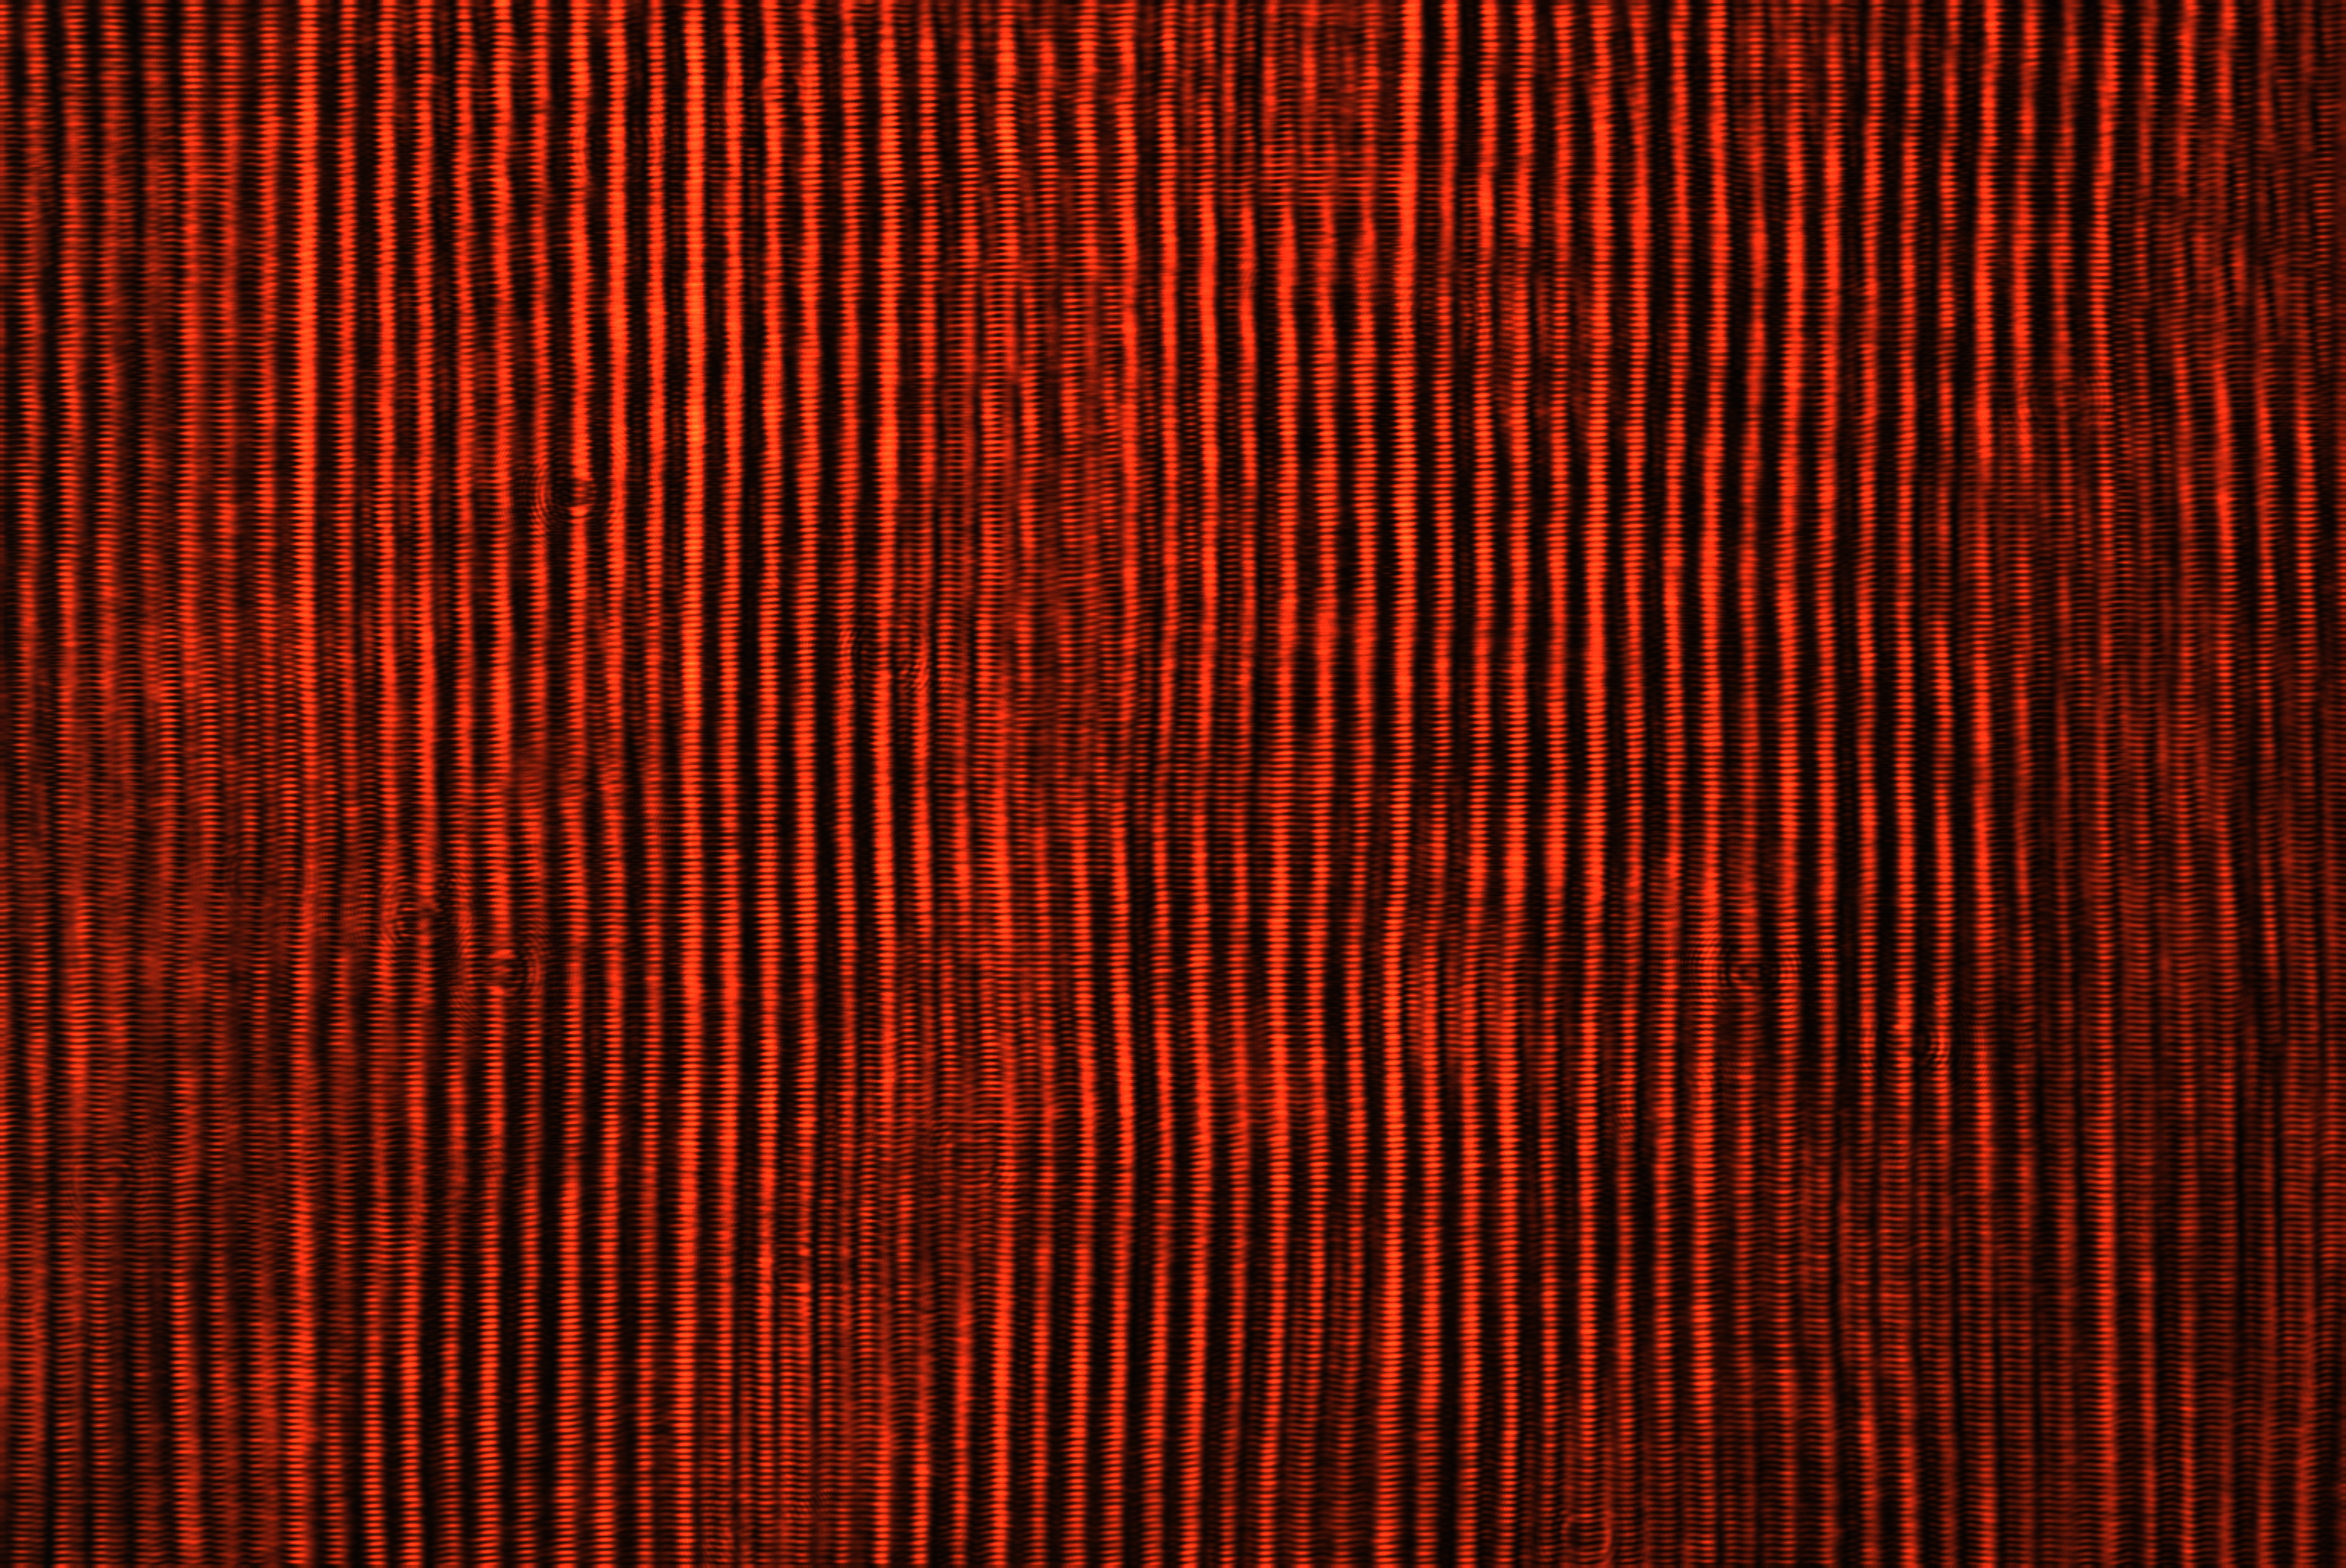
\includegraphics[width=0.6\textwidth]{chua_sim/1.png}
	\caption{第一次单涡旋吸引因子}	
\end{figure}

与仿真结果类似,调节Rk过程中也未出现第二次单涡旋吸引因子。

\subsubsection*{数据分析}
仿真和实际电路不同相图时Rk阻值见表2:

\begin{table}[H]
	\centering{
	  \begin{tabular}{ccccc}
	   \toprule
		\multicolumn{1}{l}{实验方式} & \multicolumn{1}{l}{直线} & \multicolumn{1}{l}{极限环} & \multicolumn{1}{l}{双吸引子} & \multicolumn{1}{l}{第一次单吸引子} \\
	  \midrule
		仿真电路     & 0  & 1040 & 1560  & 1601.2\\
	  全真电路    & 0 & 1018  & 1563.2  & 1661 \\
	  \bottomrule
	  \end{tabular}}
	\caption{仿真和实际电路不同相图时Rk阻值(单位:$\Omega$)}
	\label{tab:2}%
\end{table}%

经配对T检验得t值为-0.587714318298662,对应P值为0.598032391735953>0.05,无统计学差异,故得出结论仿真可以较好的模拟真实的第二种蔡氏混沌电路。

\subsection{洛伦兹混沌电路}
\subsubsection{数值模拟}

在vscode编译器中使用Jupyter Notebook, 用Python语言编写洛伦兹混沌方程:
\[\left\{
\begin{aligned}
&\frac{dx}{d\tau}=-10x+10y \\
&\frac{dy}{d\tau}=28x-y-xz \\
&\frac{dz}{d\tau}=-\frac{8}{3}z+xy
\end{aligned}
\right.
\]
此时系统处在混沌状态,该三维图\ref{fig:lorenz_3d}在 XY 平面的投影如图\ref{fig:lorenz_xy}所示,
在 XZ 平面的投影如图\ref{fig:lorenz_xz}所示,在 YZ 平面的投影如图\ref{fig:lorenz_yz}所示,
时域图为图\ref{fig:lorenz_wave},可以观察到经典的洛伦兹双吸引子(蝴蝶)曲线。

\begin{figure}[H]
	\centering
	\subfloat[三维相图]{\label{fig:lorenz_3d}
	\includegraphics[width=0.3\textwidth]{fig/lo-xyz.png}
	}%
	\subfloat[时域图]{\label{fig:lorenz_wave}
	\includegraphics[width=0.3\textwidth]{fig/lorenz_wave.png}
	}%

	\subfloat[x-y相图]{\label{fig:lorenz_xy}
	\includegraphics[width=0.3\textwidth]{fig/lo-xy.png}
	}%
	\subfloat[x-z相图]{\label{fig:lorenz_xz}
	\includegraphics[width=0.3\textwidth]{fig/lo-xz.png}
	}%
	\subfloat[y-z相图]{\label{fig:lorenz_yz}
	\includegraphics[width=0.3\textwidth]{fig/lo-yz.png}
	}%
	\caption{数值模拟相图}
	\label{fig:lorenz}
\end{figure}

\subsubsection{洛伦兹混沌电路LTspice仿真}
使用LTspice软件搭建洛伦兹混沌电路,调节R2阻值可以得到不同相图。

(1)直线

此时$R2=1\Omega$,仿真电路如下图:
\begin{figure}[H]
	\centering
	\includegraphics[width=0.4\textwidth]{fig/lo_line_cir.png}
	\caption{直线相图仿真电路}
\end{figure}

在 XY 平面的投影如图\ref{fig:lorenz_line_xy}所示,
在 XZ 平面的投影如图\ref{fig:lorenz_line_xz}所示,在 YZ 平面的投影如图\ref{fig:lorenz_line_yz}所示,
时域图为图\ref{fig:lorenz_line_wave}。

\begin{figure}[H]
	\centering
	\subfloat[x-y相图]{\label{fig:lorenz_line_xy}
	\includegraphics[width=0.4\textwidth]{fig/lo_line_xy.png}
	}%
	\subfloat[x-z相图]{\label{fig:lorenz_line_xz}
	\includegraphics[width=0.4\textwidth]{fig/lo_line_xz.png}
	}%

	\subfloat[y-z相图]{\label{fig:lorenz_line_yz}
	\includegraphics[width=0.4\textwidth]{fig/lo_line_yz.png}
	}%
	\subfloat[时域图]{\label{fig:lorenz_line_wave}
	\includegraphics[width=0.4\textwidth]{fig/lo_line_wave.png}
	}%
	\caption{直线仿真}
	\label{fig:lorenz_line}
\end{figure}

(2)双涡旋吸引因子

此时$R2=100k\Omega$,仿真电路如下图:
\begin{figure}[H]
	\centering
	\includegraphics[width=0.4\textwidth]{fig/lorenz-sim.png}
	\caption{双吸引子仿真电路}	
\end{figure}

在 XY 平面的投影如图\ref{fig:lorenz_2_xy}所示,
在 XZ 平面的投影如图\ref{fig:lorenz_2_xz}所示,在 YZ 平面的投影如图\ref{fig:lorenz_2_yz}所示,
时域图为图\ref{fig:lorenz_2_wave}。

\begin{figure}[H]
	\centering
	\subfloat[x-y相图]{\label{fig:lorenz_2_xy}
	\includegraphics[width=0.4\textwidth]{fig/lorenz_xy}
	}%
	\subfloat[x-z相图]{\label{fig:lorenz_2_xz}
	\includegraphics[width=0.4\textwidth]{fig/lorenz_xz.png}
	}%

	\subfloat[y-z相图]{\label{fig:lorenz_2_yz}
	\includegraphics[width=0.4\textwidth]{fig/lorenz_yz.png}
	}%
	\subfloat[时域图]{\label{fig:lorenz_2_wave}
	\includegraphics[width=0.4\textwidth]{fig/lorenz_double_wave.png}
	}%
	\caption{双吸引子仿真}
	\label{fig:lorenz_2}
\end{figure}

(3)单涡旋吸引因子

此时$R2=640k\Omega$,仿真电路如下图:

\begin{figure}[H]
	\centering
	\includegraphics[width=0.4\textwidth]{fig/lo_1_cir.png}
	\caption{单吸引子仿真电路}
\end{figure}

在 XY 平面的投影如图\ref{fig:lorenz_1_xy}所示,
在 XZ 平面的投影如图\ref{fig:lorenz_1_xz}所示,在 YZ 平面的投影如图\ref{fig:lorenz_1_yz}所示,
时域图为图\ref{fig:lorenz_1_wave}。

\begin{figure}[H]
	\centering
	\subfloat[x-y相图]{\label{fig:lorenz_1_xy}
	\includegraphics[width=0.4\textwidth]{fig/lo_1_xy.png}
	}%
	\subfloat[x-z相图]{\label{fig:lorenz_1_xz}
	\includegraphics[width=0.4\textwidth]{fig/lo_1_xz.png}
	}%

	\subfloat[y-z相图]{\label{fig:lorenz_1_yz}
	\includegraphics[width=0.4\textwidth]{fig/lo_1_yz.png}
	}%
	\subfloat[时域图]{\label{fig:lorenz_1_wave}
	\includegraphics[width=0.4\textwidth]{fig/lo_1_wave.png}
	}%
	\caption{单吸引子仿真}
	\label{fig:lorenz_1}
\end{figure}

\section{讨~~~论}
在蔡氏混沌电路的仿真电路和全真电路中,并没有测量非线性伏安特性曲线电阻的阻值变化,故数值仿真时缺少
关键数据$M_a$和$M_b$。此处数值计算并不能很好的与仿真电路和全真电路对应,故调节参数$M_a$、$M_b$、$\alpha$和$\beta$,
得到不同相图,仅表示蔡氏电路混沌状态时相图有直线、极限环、双吸引子、第一次单吸引子和第二次单吸引子五种,并不参与与仿真电路 和全真电路的对比之中。
若实验中测量非线性电阻曲线,并拟合成函数,则可带入完成精确的数值模拟。

在第二种蔡氏电路的模拟中,其混沌方程与第一种共用,但是由于非线性电阻的改变,第二种蔡氏电路混沌相图并不能出现第二次单吸引子。

在洛伦兹混沌电路的模拟中,数值模拟仅代入了最常见的双吸引子图像参数,仿真时也仅仅调节了R2的阻值,出现了直线,双吸引子和第一次单吸引子的图像,
若调节不同电阻或电容,有可能出现更多不同种类的相图。

关于误差分析,由于数值模拟和仿真建立在精确的计算机计算上,所以最主要的误差来源于全真电路。首先选用的电阻和电容阻值与计算仿真略有误差,其次电路的接线方法
会在一定程度上影响电路的灵敏性,例如电路中布置大量导线会增大电路断路的几率。


\section{结~~~论}
本实验采用数值计算、仿真实验和全真电路三种方式从理论和实践上还原了混沌电路。

首先,本实验探究了不含电容蔡氏电路的不同混沌状态,从Python的数值模拟上看,第一种蔡氏电路可以得到直线、极限环、双吸引子、第一次和第二次
单吸引子五种相图。通过Multisim仿真,分别取R7为0、1536、1736、1896和1920$\Omega$,可以得到这五种相图。通过搭建真实电路,使用NI Virtualbench
可以发现当滑动变阻器阻值为0、1498.2、1880.32、1907.20、1979.10$\Omega$时分别出现五种相图。使用配对T检验可以得到t值为-1.12901974098575,对应P值为0.322013731315691>0.05,无统计学差异,
故得出结论仿真可以较好的模拟真实的第一种蔡氏混沌电路。

其次,我们对含电容的蔡氏混沌电路进行Multisim仿真,发现Rk取0、1040、1560、1601.2 $\Omega$时分别出现直线、极限环、双吸引子和第一次单吸引子相图。
通过搭建真实电路,使用NI Virtualbench ,可以发现当滑动变阻器阻值为 0、1018、1563.2和1661 $\Omega$时出现这四种相图。
经配对T检验得t值为-0.587714318298662,对应P值为0.598032391735953>0.05,无统计学差异,故得出结论仿真可以较好的模拟真实的第二种蔡氏混沌电路。

最后,我们使用Python对经典洛伦兹混沌方程进行模拟,得到双吸引子的三维图、时域图和各平面投影图。使用LTspice仿真,当R2为1、100k、640k$\Omega$时,
洛伦兹混沌电路的相图分别为直线、双吸引子和第一次单吸引子。若调节更多原件的参数,可能可以得到更多种类的相图。

\newpage
% \renewcommand\refname{参考文献}
% \bibliographystyle{chinese}
% \bibliography{ref}

\printbibliography[title=参考文献] 
\clearpage

	
\section*{\LARGE 附录A}
\section*{【思考题】}
\subsection*{1. 检索资料,简述混沌电路的可能应用。要求给出参考文献。}
\subsubsection*{保密通信}
由于混沌振荡频谱既有貌似随机又有宽频带连续频谱,在无线电通信上很适合用于保密通信与扩频通信。
要利用混沌进行保密通信,要求保密通信双方必须有完全相同的非线性电路(混沌电路),
这样才能达到混沌同步,从而实现保密信号从发射机的编码到接收机解码的全过程.否则无法达到混沌同步,
无法解密信息与信号,也就无法进行保密通信。混沌通信方式多种多样,但其基本思路是相同的,
即把被传输的信息源加在某一由混沌系统产生的混沌信号上,生成混合类噪声信号,对信号源加密,该信号发送到接收器上后,
再由一相应的的混沌系统分离其中的混沌信号,即解密过程,进而恢复出原输送的信息源。由于混沌同步效应的存在,使得这一解密过程能够实现\autocite{S1}。
\subsubsection*{温度测量}
作者给出了一种基于映射式混沌电路的温度测量新方法,与现有的测量方法完全不同。
把对温度敏感的所有元件参数都考虑在内,测量过程中将这些元件都置于测温环境中,电路输出的符号序列直接反映了温度的变化。
因此不再有测量电路的温度漂移的问题,具有较高的精确度和灵敏度。
此外,该电路的结构简单,又能直接输出反映温度变化的二进制代码,即数字信号,便于计算机处理。计算机仿真和实际电路实验都显示该方法的优越性\autocite{S2}。

\newpage
\section*{\LARGE 附录B}
\section*{【代码页】}
\subsection*{蔡氏电路数值模拟代码}
\begin{lstlisting}
	import numpy as np
	import matplotlib.pyplot as plt
	from scipy.integrate import ode

	def Chua(M1, M2, alpha, beta, axis):
    # Define the ODE
    h = lambda x: M2*x + (M1-M2)*(abs(x+1)-abs(x-1))/2
    def derivative(t, v, d):
        dxdt = alpha * (v[1] - v[0] - h(v[0]))
        dydt = v[0] - v[1] + v[2]
        dzdt = - beta * v[1]
        return [dxdt, dydt, dzdt]
    # ODE solver
    v0 = [0.7, 0.0, 0.0]
    t0 = 0.0
    r = ode(derivative).set_integrator('dopri5')
    r.set_initial_value(v0, t0).set_f_params(1)
    # Time series
    tmax = 50
    dt = 0.02
    num_steps = int(tmax / dt) + 2
    # Generate the trace
    x = np.zeros(num_steps - 1)
    y = np.zeros(num_steps - 1)
    z = np.zeros(num_steps - 1)
    x[0], y[0], z[0] = v0
    idx = 1
    while r.successful() and r.t < tmax:
        r.integrate(r.t+dt)
        x[idx], y[idx], z[idx] = r.y[0:3]
        idx += 1
    
    # Plot
    plt.figure(figsize= (9, 6))

    if axis == "x-y":
        plt.plot(x, y, color='lightseagreen', 
                        label='M1 = {:.1f}, M2 = {:.1f}, alpha = {:.1f}, beta = {:.1f}'
                        .format(M1, M2, alpha, beta))
        plt.xlabel('x')
        plt.ylabel('y')
        plt.grid()
        plt.legend(loc='center left', bbox_to_anchor=(0.2, -0.15))
    elif axis == "x-z":
        plt.plot(x, z, color='lightseagreen', 
                        label='M1 = {:.1f}, M2 = {:.1f}, alpha = {:.1f}, beta = {:.1f}'
                        .format(M1, M2, alpha, beta))
        plt.xlabel('x')
        plt.ylabel('z')
        plt.grid()
        plt.legend(loc='center left', bbox_to_anchor=(0.2, -0.15))     
    elif axis == "y-z":
        plt.plot(y, z, color='lightseagreen', 
                        label='M1 = {:.1f}, M2 = {:.1f}, alpha = {:.1f}, beta = {:.1f}'
                        .format(M1, M2, alpha, beta))
        plt.xlabel('y')
        plt.ylabel('z')
        plt.grid()  
        plt.legend(loc='center left', bbox_to_anchor=(0.2, -0.15))  
    elif axis == "3d":
        fig = plt.figure(figsize= (9, 6))
        ax = fig.add_subplot(projection='3d')
        plt.plot(x, y, z, color='lightseagreen', 
                            label='M1 = {:.1f}, M2 = {:.1f}, alpha = {:.1f}, beta = {:.1f}'
                            .format(M1, M2, alpha, beta))
        ax.set_xlabel('x')     
        ax.yaxis.set_label_text('y')
        ax.zaxis.set_label_text('z')
        plt.legend(loc='center left', bbox_to_anchor=(0.2, -0.15))  
        plt.grid()   
    elif axis == "wave":
        fig, ax =  plt.subplots(3, 1, figsize=(9, 6))
        ax[0].plot(x, color='lightseagreen')
        ax[0].set_xlabel('Time t/s')
        ax[0].set_ylabel('x')
        ax[0].grid()

        ax[1].plot(y, color='lightseagreen')
        ax[1].set_xlabel('Time t/s')
        ax[1].set_ylabel('y')
        ax[1].grid()

        ax[2].plot(z, color='lightseagreen')
        ax[2].set_xlabel('Time t/s')
        ax[2].set_ylabel('z')
        ax[2].grid()
        plt.subplots_adjust(left=None, bottom=None, right=None, top=None, wspace=0.2, hspace=0.2)

		#line
		for axis in ['x-y', 'y-z', 'x-z', '3d', 'wave']:
		Chua(M1=-2.0, M2=-1.3, alpha=26, beta=12, axis=axis)

		#limit circle
		for axis in ['x-y', 'y-z', 'x-z', '3d', 'wave']:
        Chua(M1=-0.5, M2=1.0, alpha=13, beta=13, axis=axis)

		#double attractors
		for axis in ['x-y', 'y-z', 'x-z', '3d', 'wave']:
		Chua(M1=-1.1, M2=-0.7, alpha=21, beta=36, axis=axis)

		#2st single attractor
		for axis in ['x-y', 'y-z', 'x-z', '3d', 'wave']:
		Chua(M1=-1.1, M2=-0.7, alpha=21, beta=31.3, axis=axis)

		#2nd single attractor
		for axis in ['x-y', 'y-z', 'x-z', '3d', 'wave']:
		Chua(M1=-1.1, M2=-0.7, alpha=21, beta=150, axis=axis)
\end{lstlisting}

\subsection*{洛伦兹系统数值模拟代码}
\begin{lstlisting}
	import numpy as np
	from scipy import integrate
	import matplotlib.pyplot as plt
	from mpl_toolkits.mplot3d import Axes3D

	def lorenz(p,t,s,r,b):
	x,y,z = p.tolist()          #无质量点的当前位置(x,y,z)
	print("x,y,z,t:",x,y,z,t)   #帮助理解odeint的执行过程
	return s*(y-x),x*(r-z)-y,x*y-b*z #返回dx/dt,dy/dt,dz/dt

	t = np.arange(0,100,0.01)
	track = integrate.odeint(lorenz,(0.0,1.00,0.0),t,args=(10.0,28.0,2.6))
	#track2 = integrate.odeint(lorenz,(0.0,1.01,0.0),t,args=(10.0,28.0,2.6))
	#print("type(track):",type(track),"track.shape:",track.shape)

	fig = plt.figure(figsize=(12,6))
	ax = fig.gca(projection='3d')   #获取当前子图,指定三维模式
	ax.plot(track[:,0],track[:,1],track[:,2],lw=1.0,color='r')	#画轨迹			
	ax.set_xlabel('x')
	ax.set_ylabel('y')
	ax.set_zlabel('z')
	plt.show()

	plt.plot(track[:,0], track[:,1])
	plt.xlabel('x')
	plt.ylabel('y')
	plt.show()

	plt.plot(track[:,0], track[:,2])
	plt.xlabel('x')
	plt.ylabel('z')
	plt.show()

	plt.plot(track[:,1], track[:,2])
	plt.xlabel('y')
	plt.ylabel('z')
	plt.show()

	fig2, axs = plt.subplots(3, sharex=True)
	fig2.suptitle('x, y and z against t')
	axs[0].plot(t, track1[:,0])
	axs[1].plot(t, track1[:,1])
	axs[2].plot(t, track1[:,2])

	axs[0].set(ylabel = 'x')
	axs[1].set(ylabel = 'y')
	axs[2].set(ylabel = 'z')

	axs[1].set(xlabel = 't')

	axs[0].set_ylim(-20, 20)
	axs[1].set_ylim(-25, 25)
	axs[2].set_ylim(5, 50)

	plt.xticks(np.arange(min(t), max(t)+1, 10))
	plt.show()
\end{lstlisting}


\end{document}
